\documentclass{article}
\usepackage[T1,T2A]{fontenc}
\usepackage[utf8]{inputenc}
\usepackage[english,russian]{babel}

\usepackage[left=3cm,right=3cm,
    top=3cm,bottom=3cm,bindingoffset=0cm]{geometry}

\usepackage{graphicx}
\usepackage{color}
\usepackage{hyperref}
\usepackage{amsmath}
\usepackage{amsfonts}
\usepackage{amssymb}


\usepackage{setspace}
\usepackage{indentfirst}
\usepackage{textcomp}
\usepackage{ifthen}
\usepackage{calc}
\usepackage{mathrsfs}
\usepackage[dvipsnames]{xcolor}


\title{Введение в машинное обучение}
\author{Национальный исследовательский университет "Высшая школа экономики" \and Yandex School of Data Analysis\\\\
Неофициальный конспект по курсу.}

\begin{document}
\maketitle

\section{Решающие деревья}

\subsection{Описание метода}
\textbf{Решающие деревья} --- это целый класс методов машинного обучения.
\\

Эти методы предназначены исходно для решения задач классификации, очень редко для задач регрессии. Изначально решающие деревья возникли как попытка \textbf{формализовать человеческое мышление} при принятии решений.
\\

Например, решающим деревом мы можем описать рассуждения врача, который за 5-6 вопросов отбирает нужные признаки и может поставить некоторый диагноз. При этом какие-то признаки исключают друг друга и целые группы симптомов, отсюда и получается \textit{дерево}.

Конечно, на практике не все так просто, но все же.

\subsection{Задача классификации (обучение с учителем)}

Напомним, что в общем случае мы занимаемся задачами обучения с учителем:

\begin{center}
\line(1,0){400}
\end{center}

\begin{itemize}

\item[] Задача восстановления зависимости $\quad y: X\rightarrow Y$, $|Y| < \infty$\\
		по точкам обучающей выборки $(x_i, y_i), i = 1,\ldots, l$.

\item[] \textbf{Дано:} векторы $x_i = (x_i^1, \ldots, x_i^n)$ --- объекты обучающей выборки\\
		$y_i = y(x_i)$ --- классификации, ответы учителя, $(i = 1, \ldots, l)$
		
		$$
		\begin{pmatrix}
			x_1^1 & \ldots & x_1^n)\\
			\ldots & \ldots & \ldots\\
			x_l^1 & \ldots & x_l^n)\\
		\end{pmatrix}
		\xrightarrow{y*}
		\begin{pmatrix}
			y_1\\
			\ldots\\
			y_l
		\end{pmatrix}
		$$
		
\item [] \textbf{Найти:} функцию \textcolor{red}{$a(x)$}, способную классифицировать объекты произвольной тестовой выборки $\tilde{x}_i = (\tilde{x}_i^1, \ldots, \tilde{x}_i^n)$, $i = 1, \ldots, k$:

		$$
		\begin{pmatrix}
			\tilde{x}_1^1 & \ldots & \tilde{x}_1^n)\\
			\ldots & \ldots & \ldots\\
			\tilde{x}_k^1 & \ldots & \tilde{x}_k^n)\\
		\end{pmatrix}
		\xrightarrow{\textcolor{red}{a?}}
		\begin{pmatrix}
			\textcolor{red}{a(\tilde{x}_1)}\\
			\ldots\\
			\textcolor{red}{a(\tilde{x}_k)}
		\end{pmatrix}
		$$
\end{itemize}

\begin{center}
\line(1,0){400}
\end{center}

При этом в нашей задаче мы будем строить \textit{алгоритм классификации} в виде \textbf{дерева}.

\subsection{Определение бинарного решающего дерева}

\textbf{Бинарное дерево} --- это ациклический граф, в котором есть два типа вершин: либо вершина соединена с двумя дочерними (\textit{внутренний тип}), либо вершина не соединена ни с одной (\textit{листовой/терминальный тип}).
\\

\textbf{Бинарное решающее дерево} --- алгоритм классификации $a(x)$, задающийся бинарном деревом. В нем определена \textit{дополнительная} информация, связанная с каждой внутренней вершиной и каждой лиственной вершиной:

\begin{enumerate}
\item[1)] $\forall v \in V_{\text{внутр}} \rightarrow$ предикат
			$\beta_v: X \rightarrow \{0, 1\}$, $\beta_v\in \mathscr{B}$,

\item[2)] $\forall v \in V_{\text{лист}} \rightarrow$ имя класса $c_v \in Y$,

\item[] где $\mathscr{B}$ --- множество бинарных признаков или предикатов\\
		(например, вида $\beta(x) = [x^j \geqslant \theta_j]$, $x^j \in \mathbb{R}$)
\end{enumerate}

Предикат $\beta_v$ (для \textbf{внутренней} вершины $v$) способен, взяв объект, сказать, \textit{<<дальше мы отправим его в левую ветвь, или в правую ветвь дерева?>>}.

В каждой из \textbf{листовой} вершин мы будем записывать \textit{имя} или \textit{метку} одного из классов (элемент множества ответов $Y$). То есть дошли до листа --- гарантируем (в меру своих возможностей) отношение объекта к определенному классу.
\\

\textbf{Предикаты} для внутренних вершин мы берем из некоторого множества бинарных предикатов $\mathscr{B}$.

В простейшем случае, если все признаки \textit{бинарны} --- это будут просто исходные признаки.

Если признаки \textit{вещественные}, то мы будем строить предикаты в виде бинарного условия \textit{<<значение признака меньше/больше некоторого порогового значения $\theta_j$>>} (см. пример выше).
\\

\textbf{Принятие решений} нашим решающим бинарным деревом в итоге, на самом-то деле, можно описать достаточно простым алгоритмом спуска по дереву:

\begin{tabular}{ p{8cm} c }
\begin{enumerate}
\item[1:] $v := v_0$;
\item[2:] \textcolor{blue}{пока} $v \in V_{\text{внутр}}$
\item[3:] \qquad \textcolor{blue}{если} $\beta_v(x) = 1$ \textcolor{blue}{то}
\item[4:] \qquad \qquad переход вправо: $v := R_v$;
\item[5:] \qquad \textcolor{blue}{иначе}
\item[6:] \qquad \qquad переход влево: $v := L_v$;
\item[7:] \textcolor{blue}{вернуть} $c_v$.
\end{enumerate}
&
\raisebox{-\totalheight}{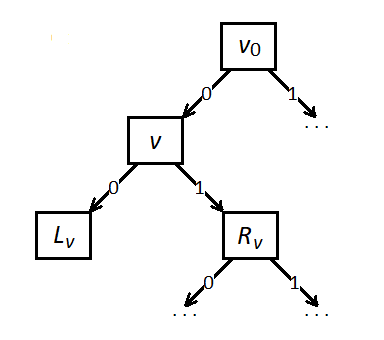
\includegraphics[scale=0.65]{images/3_1.png}}
\end{tabular}

Нам достаточно пустить объект по этому дереву, начиная с корня. В каждой вершине мы проверяем значение предиката на данном объекте, переходим в нужную ветвь, и так идем до некоторой листовой вершины, которая и говорит нам о классе объекта.

\newpage
\subsubsection{Пример. Задача Фишера}

Задача Фишера (классическая задача) о классификации цветков ириса на 3 класса. В выборке по 50 объектов каждого класса, имеется 4 признака:

\begin{center}
    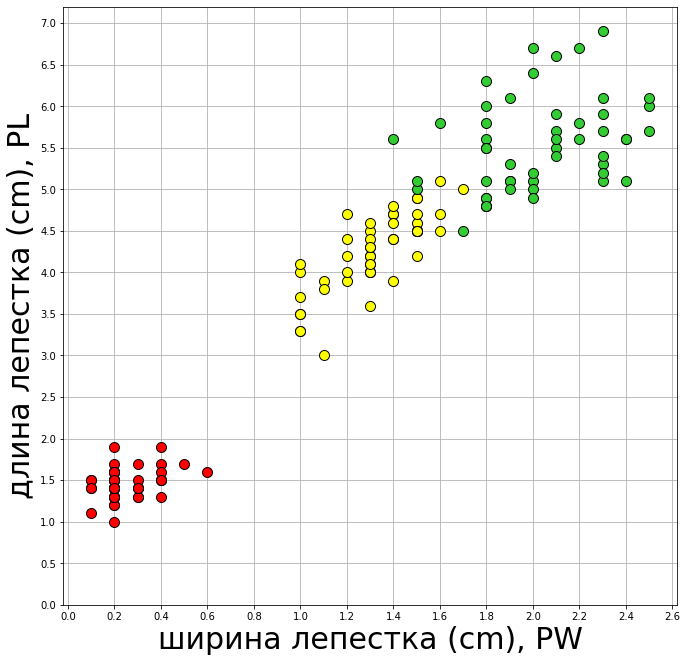
\includegraphics[scale=0.4]{images/3_2.png}
\end{center}

\textbf{На графике:}

в осях двух самых информативных признаков (из 4)

два класса разделились без ошибок, на третьем 3 ошибки.
\\

Гладя на эту картинку можно в принципе вручную построить \textbf{решающее бинарное дерево}:

\begin{enumerate}
\item Отсекаем тот класс, который лежит в нижней области --- $PL < 2.5$;
\item Отсекаем правую часть множества зеленых точек --- $PW > 1.68$;
\item Осталось отделить желтые от нескольких зеленых. Заметим, что для желтых (большинства выполняется условие $PL < 5$.
\end{enumerate}

Таким образом:

\begin{center}
    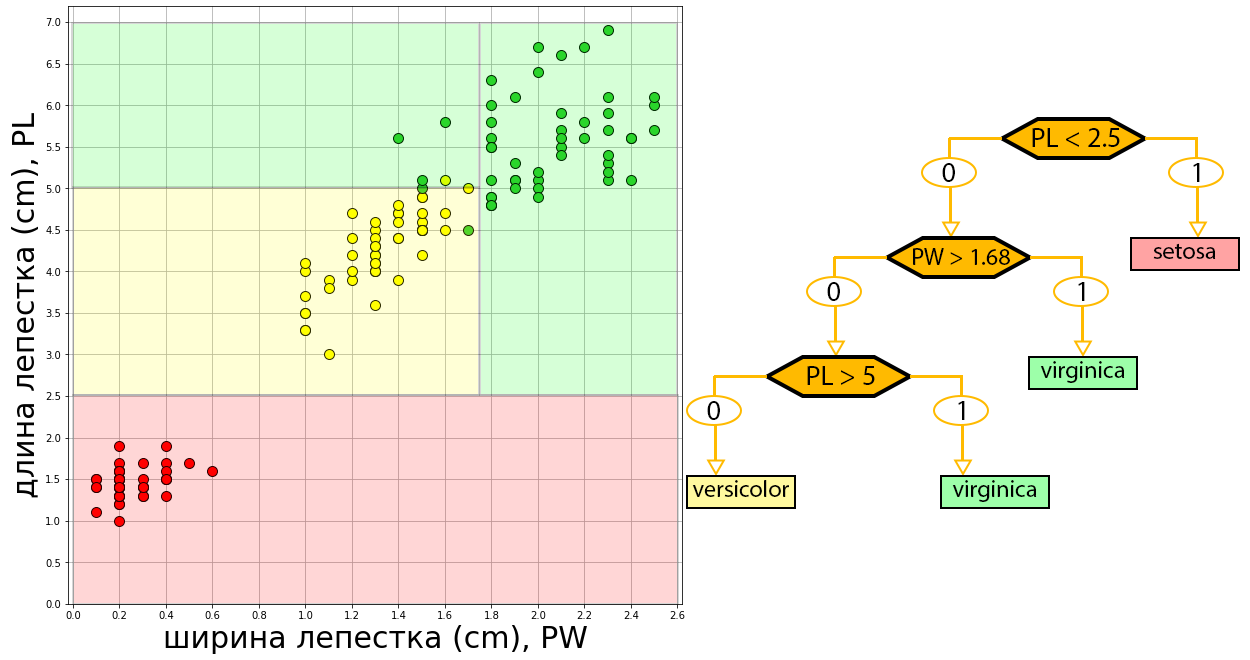
\includegraphics[scale=0.35]{images/3_3.png}
\end{center}

Итого 3 шага для того, чтобы представить алгоритм классификации в виде решающего дерева.

Можно заметить, что при таком алгоритме у нас получилось 3-4 ошибки.
\\

\textbf{Замечание.} Существует и альтернативный способ представления решающего дерева в виде списка правил:
\\

\begin{tabular}{l l}
\fcolorbox{black}{red!40}{ setosa } & $r_1(x) = [PL \leqslant 2.5]$\\
\\
\fcolorbox{black}{green!40}{virginica} & $r_2(x) = [PL > 2.5] \wedge [PW > 1.68]$\\
\\
\fcolorbox{black}{green!40}{virginica} & $r_3(x) = [PL > 5] \wedge [PW \leq 1.68]$\\
\\
\fcolorbox{black}{yellow!40}{versicolor} & $r_4(x) = [PL > 2.5] \wedge [PL \leq 5] \wedge [PW < 1.68]$
\end{tabular}
\\

Дерево нам разделило пространство двух признаков на 4 не пересекающиеся области, а их мы можем описать условиями, которые их и ограничивают.

Такие правила называются \textbf{логическими закономерностями}, и часто они характеризуются тем, что каждое такое правило выделяет какую-то область в пространстве объектов, где содержатся объекты только одного класса или преимущественно одного класса.

\newpage
\subsection{Алгоритм построения решающего дерева}

\begin{itemize}
\item \textbf{Жадный алгоритм построения дерева ID3}
\end{itemize}

Классическая процедура для построения решающего дерева \textbf{ID3 --- Induction of Decision Tree}:

\begin{center}
\line(1,0){400}
\end{center}

\begin{itemize}
\item[1:] \textcolor{blue}{LearnID3} ($U \subseteq X^l$);

\item[2:] \textcolor{blue}{если}
				все объекты из $U$ лежат в одном классе $c \in Y$
			\textcolor{blue}{то}

\item[3:] \qquad \textcolor{blue}{вернуть} новый лист $v, c_v := c$;

\item[4:] \textcolor{red}{найти предикат с максимальной информативностью:}\newline
		\textcolor{red}{$\beta := arg\ \underset{\beta \in \mathscr{B}}{max}\ I(\beta, U)$};
			
\item[5:] разбить выборку на две части $U = U_0 \sqcup U_1$ по предикату $\beta$:\newline
			 $U_0 := \{x \in U: \beta(x) = 0\}$\newline
			 $U_0 := \{x \in U: \beta(x) = 1\}$

\item[6:] \textcolor{blue}{если}
				$U_0 = \emptyset$ или $U_1 = \emptyset$
			\textcolor{blue}{то}
			
\item[7:] \qquad \textcolor{blue}{вернуть} новый лист $v, c_v :=$ Мажоритарный класс($U$);

\item[8:] создать новую внутреннюю вершину v: $\beta_v := \beta$;\newline
			 Построить левое поддерево: $L_v :=$ LearnID3($U_0$);\newline
			 Построить правое поддерево: $R_v :=$ LearnID3($U_1$);

\item[9:] \textcolor{blue}{вернуть} $v$;

\end{itemize}

\begin{center}
\line(1,0){400}
\end{center}

Разберем алгоритм по пунктам:

\begin{itemize}
\item Программа принимает на вход некоторую подвыборку обучающей выборки. В первый раз (процедура рекурсивная) мы подаем на вход всю выборку:

\qquad 1: \textcolor{blue}{LearnID3} ($U \subseteq X^l$);

\item Если все объекты в подвыборке оказались одного класса, мы можем вернуть из процедуры лист (дальше классифицировать некуда; куда этот лист девается --- об этом дальше):

\qquad 2: \textcolor{blue}{если}
				все объекты из $U$ лежат в одном классе $c \in Y$
			\textcolor{blue}{то}

\qquad 3: \qquad \textcolor{blue}{вернуть} новый лист $v, c_v := c$;

\item Дальше самый важный шаг. На этом этапе мы имеем выборку, в которой точно находятся объекты разных классов (мы только что проверили обратный случай). Попытаемся найти предикат, который максимально хорошо выделял бы нам объекты какого-то одного класса, или просто отделял их совсем от других классов.

Для того, чтобы определить, насколько предикат информативный, существует множество \textbf{критериев информативности} -- в данном случае обозначается как $I$. В общем-то именно из-за выбора критерия информативности возникает большое разнообразие методов построения решающих деревьев.

\qquad 4: \textcolor{red}{найти предикат с максимальной информативностью:}

\qquad \textcolor{red}{$\beta := arg\ \underset{\beta \in \mathscr{B}}{max}\ I(\beta, U)$};

\item Так как мы строим бинарное дерево, и предикаты у нас тоже бинарные, мы можем спокойно разделить нашу выборку на две подвыборки --- для одной предикат будет выполняться, для другой нет:

\qquad 5:  разбить выборку на две части $U = U_0 \sqcup U_1$ по предикату $\beta$:

\qquad \qquad 			 $U_0 := \{x \in U: \beta(x) = 0\}$

\qquad \qquad 			 $U_0 := \{x \in U: \beta(x) = 1\}$

\item На всякий случай проверим, а не получилась ли одна из подвыборок пустой. Если такое случится, это будет значит, что \textit{несмотря на то}, что в подвыборке $U$ были объекты \textit{разных} классов, мы \textit{не смогли} найти предикат, который как-либо разделил бы их.

Нужно вводить новые предикаты, но это уже не задача алгоритма построения дерева, да и не всегда возможно (ошибки могут быть всегда), поэтому тут мы вернем новую листовую вершину, которой присвоим преобладающий в этой подвыборке класс (которого больше всего).

\qquad 6: \textcolor{blue}{если}
				$U_0 = \emptyset$ или $U_1 = \emptyset$
			\textcolor{blue}{то}
			
\qquad 7: \qquad \textcolor{blue}{вернуть} новый лист $v, c_v :=$ Мажоритарный класс($U$);

\item К этому моменту мы можем гарантировать, что обе подвыборки не пустые, поэтому мы можем создать внутреннюю вершину, которой присвоим наш разделивший выборку предикат. К этой вершине мы можем построить две ветви, которые будут строиться рекурсивно из наших подвыборок:

\qquad 8: создать новую внутреннюю вершину v: $\beta_v := \beta$;

\qquad \qquad	Построить левое поддерево: $L_v :=$ LearnID3($U_0$);

\qquad \qquad	Построить правое поддерево: $R_v :=$ LearnID3($U_1$);

\item Поддеревья готовы, вершина подготовлена, можем ее спокойно вернуть из процедуры:

\qquad 9: \textcolor{blue}{вернуть} $v$;

\end{itemize}

\subsubsection{Варианты критериев ветвления}

Рассмотрим все же, какие бывают \textbf{критерии ветвления} \textit{(информативности)}:

\begin{itemize}
\item \textbf{Критерий Джини:}

$$I(\beta, X^l) = \#\{(x_i, x_j):\ (y_i = y_j) \text{ и } (\beta(x_i) = \beta(x_j))\}.$$

Он показывает, сколько есть пар объектов, лежащих в одном и том же классе, которые вместе идут в одну из дочерних вершин. У этих объектов должны совпадать метки классов и значения предикатов.

По сути критерий измеряет то, насколько часто объекты одних классов объединяются.

\item $D$\textbf{-критерий В.И.Донского:}

$$I(\beta, X^l) = \#\{(x_i, x_j):\ (y_i \not=y_j) \text{ и } (\beta(x_i) \not= \beta(x_j))\}.$$

По сути просто противоположная критерию Джини стратегия --- подсчитываем число пар объектов, которые лежали в разных классах и они ушли в разные ветви.

По сути измеряет, насколько данный предикат обладает способностью разделять объекты разных классов.

\item Энтропийный критерий:

$$I(\beta, X^l) = 
\sum\limits_{c \in Y} h\Biggl(\frac{P_c}{l}\Biggr)
- \frac{p}{l}h\Bigl(\frac{p_c}{p}\Bigr)
- \frac{l - p}{l}h\Biggl(\frac{P_c - p_c}{l - p}\Biggr),$$

где $h(z) = -z log_2(z)$,

$P_c(X^l) = \#\{x_i:\ y_i = c\}$,

$p_c(X^l) = \#\{x_i:\ (y_i = c) \text{ и } (\beta(x_i) = 1)\}$,

$p(X^l) = \#\{x_i:\ \beta(x_i) = 1\}$,
\\

Достаточно сложный, поэтому разбирать его не будем. Впрочем, на практике часто оказывается, что этот критерий очень похож на критерий Джини и работает примерно так же...

\end{itemize}

\subsection{Обработка пропусков}

При построении решающих деревьев часто появляется важная проблема -- \textbf{пропуски в данных}.

Если возвращаться к примеру с врачом и пациентом, то пациент так и может ответить: \textit{<<Я не знаю>>}. Так и мы будем обращаться к признаку объекта и просто не сможем получить ответ на свой вопрос. 

И вот решающие деревья достаточно удобно и эффективно, как мы потом увидим, решают эту проблему.
\\

Чтобы решить проблему с пропусками, нам понадобится сделать некоторые уточнения как на стадии обучения, так и на стадии классификации:

\begin{enumerate}
\item [] \textbf{На стадии обучения:}

	\begin{itemize}
	\item $\beta_v(x)$ не определено $\Rightarrow x_i$ \textbf{исключается} из $U$ для $I(\beta, U)$.
	\\
	
	Таким образом "информативность" предиката будет вычисляться без этого \textit{объекта} (важно, что именно объекта!, а не исключение признака для всех объектов).
	\\
	
	\item $q_v = \frac{|U_0|}{|U|}$ --- оценка \textbf{вероятности} левой ветви (попадания в левую ветвь),
			$\forall v \in V_\text{внутр}$.
	\\
		
	Вероятность для правой ветви, очевидно, всегда находится как $1 - q_v$. Зачем это вообще нужно? Увидим дальше на этапе классификации.
	\\
	
	\item $P(y |\ x, v) = \frac{1}{|U|}\#{x_i \in U:\ y_i = y}$ для всех $v \in V_\text{лист}$.
	\\
		
	По сути это функция-интерпретация \textbf{условной вероятности} для листовых вершин --- условная вероятность класса $y$ для данного объекта $x$, который дошел до листовой вершины $v$. По сути просто доля объектов обучающей выборки, которые дошли до этой вершины и принадлежат классу $y$
	
	\end{itemize}
	
\item [] \textbf{На стадии классификации}

	Мы имеем объект $x$, который пропускаем по нашему дереву сверху-вниз. Его обработка с учетом пропусков производится следующим образом:
	
	\begin{itemize}
	\item $\beta_v(x)$ \textbf{не определено} $\Rightarrow$ \textbf{пропорциональное распределение}:
	
	$$P(y |\ x,v) = q_v P(y|\ x, L_v) + (1 - q_v) P(y|\ x, R_v).$$
	
	То есть мы пропускаем объект \textit{и в левое поддерево, и в правое}. По сути мы посчитаем вероятность \textbf{каждого класса} для данного объекта $x$, дошедшего до вершины $v$, \textbf{учитывая} то, с какой вероятностью он может попасть в левое и правое поддерево --- \textbf{для этого} мы и рассчитывали $q_v$.
	
	\item $\beta_v(x)$ \textbf{определено} $\Rightarrow$ либо налево, либо направо:
	
	$$P(y|\ x, v) = \bigl(1 - \beta_v(x)\bigr)P(y|\ x, L_v) + \beta_v(x)P(y|\ x, R_v).$$
	
	То есть значение предиката определено, и объект $x$ однозначно идет либо налево, либо направо --- не забываем, что $\beta_v(x) = \{0, 1\}$, поэтому "либо то, либо то" мы контролируем домножением на $1 - \beta_v(x)$ и $\beta_v(x)$ соответственно, так как они принимают значения $\{1,0\}$. 
	
	При этом мы все еще мыслим вероятностями, чтобы получить общий удобный случай.
	
	\item Окончательное решение --- \textbf{наиболее вероятный класс}:
	
	$$a(x) = arg\ \underset{y\in Y}{max}P(y|\ x, v_0).$$
	
	В данном случае $v_0$ --- корневая вершина. То есть в процессе всего нашего обхода мы в итоге посчитаем условные вероятности для каждого класса \textbf{для корневой вершины}, и на основе этого можем выбрать класс, к которому объект, очевидно, максимально вероятно принадлежит.
	
	Этот принцип называется \textbf{<<принцип максимума апостериорной вероятности}.
	
	\end{itemize}
\end{enumerate}

Таким образом мы получаем полностью рабочую схему решающего дерева, включающего обработку пропусков.

\subsection{Достоинства и недостатки дерева ID3}

\textbf{Достоинства:}

\begin{itemize}
\item Интерпретируемость и простота классификации.

\item Гибкость: можно варьировать множество $\mathscr{B}$ (множество предикатов).

\item Допустимость разнотипных данных и данных с пропусками.
\item Трудоемкость линейна по длине выборки $O(|\mathscr{B}|hl)$ (как по признакам, так и по количеству объектов).

\item Не бывает отказов от классификации (опять же, из-за обработки пропусков).
\end{itemize}

\textbf{Недостатки} (вытекают из жадности)\textbf{:}

\begin{itemize}
\item Жадный ID3 переусложняет структуру дерева, и, как следствие, сильно переобучается.

	Решения, которые принимаются в каждой внутренней вершине дерева, локально оптимальны, но не оптимальны глобально. Полным перебором мы всегда можем найти более компактное дерево, вероятно, даже с меньшим числом ошибок.
	
\item Фрагментация выборки: чем дальше $v$ от корня, тем меньше статистическая надежность выбора $\beta_v, c_v$.

	Когда мы доходим до вершин, близких терминальным (листам), мы часто имеем дело с высокой \textit{фрагментацией} выборки, так как туда доходит \textit{небольшое} число объектов, и решения о выборе предиката или соотнесения с классом становятся \textit{статистически ненадежными}.
	
\item Высокая чувствительность к шумам, к составу выборки, к критерию информативности.

	Часто малое изменение выборки приводит к совершенно иному построению дерева: где-то выберется иначе предикат и по цепочке изменения будут идти по всему поддереву.
\end{itemize}

\newpage
\subsection{Способы устранения недостатков решающих деревьев}

Только что мы уже сказали, что основная проблема решающего дерева ID3 в \textbf{переусложнении} дерева. Посмотрим явно на эту проблему на примере синтетической задачи классификации \textit{<<задача исключающего ИЛИ>>}.

\subsubsection{Пример. Задача исключающего ИЛИ}

Данная задача не решается, например, линейным классификатором (то есть не может быть разделена прямой на два класса без ошибок), поэтому для нас она более чем подойдет.

Задача ставится однозначно: имеется логическая функция XOR. Если нарисовать точки значений в плоскости $(a, b)$, где $a$ --- первый аргумент, а $b$ --- второй, то получим:

\begin{center}
    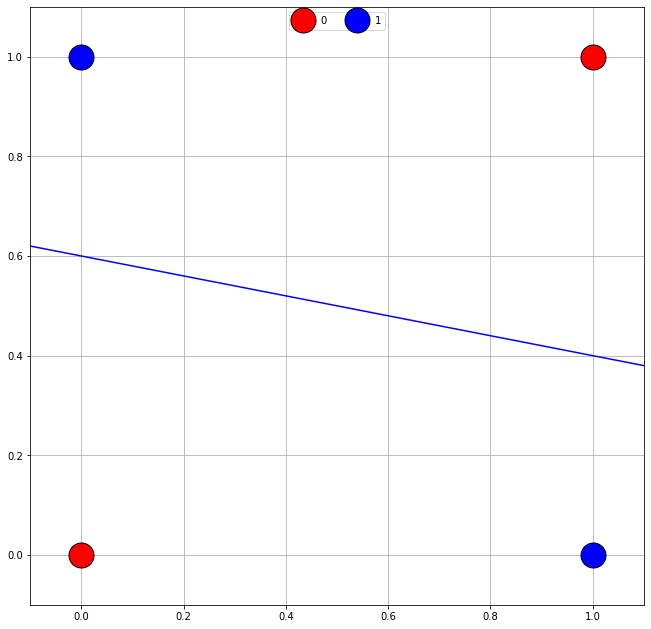
\includegraphics[scale=0.3]{images/3_4.png}
\end{center}

Линия проведена для примера, что одной линией эти случаи не разделить. Казалось бы, это все можно просто вычислить. Но если мы будем иметь какие-то объекты с вещественными признаками, которые тоже надо будет как-то классифицировать, то мы получим следующую картину:

\begin{center}
    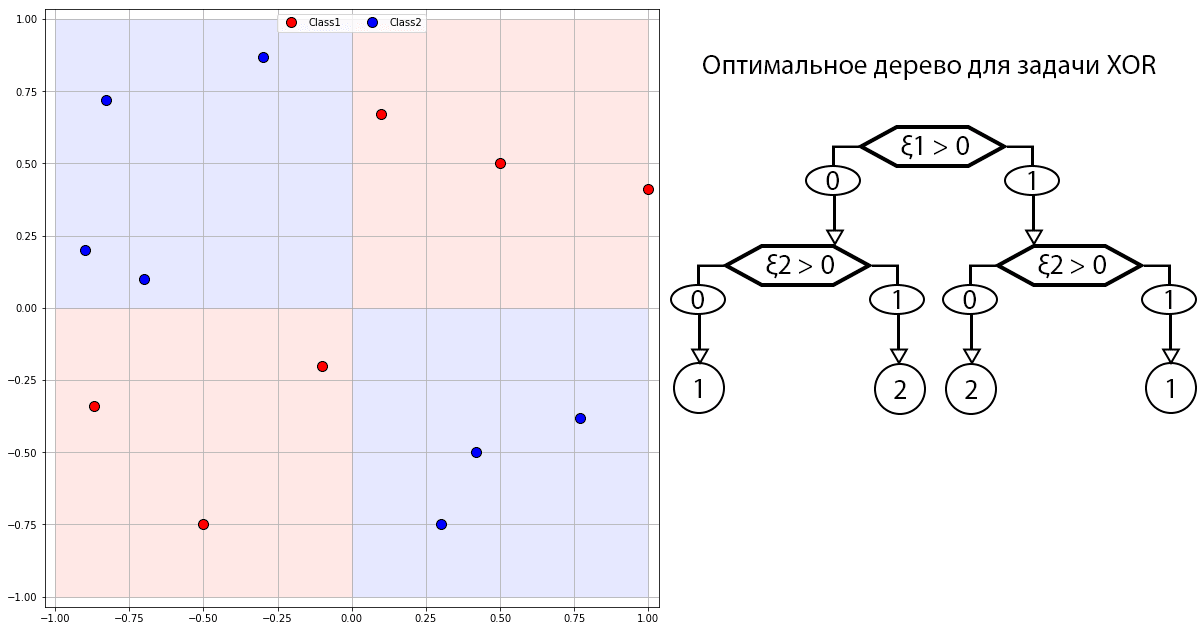
\includegraphics[scale=0.365]{images/3_5_XOR_optimal.png}
\end{center}

Соответственно, по этой картине мы можем вполне выделить оптимальное решающее дерево (там же на рисунке, если вдруг не заметно). Однако алгоритм ID3 даст нам совершенно иную картину, и не сказать, что неправильную, но уж точно не оптимизированную:

\begin{center}
    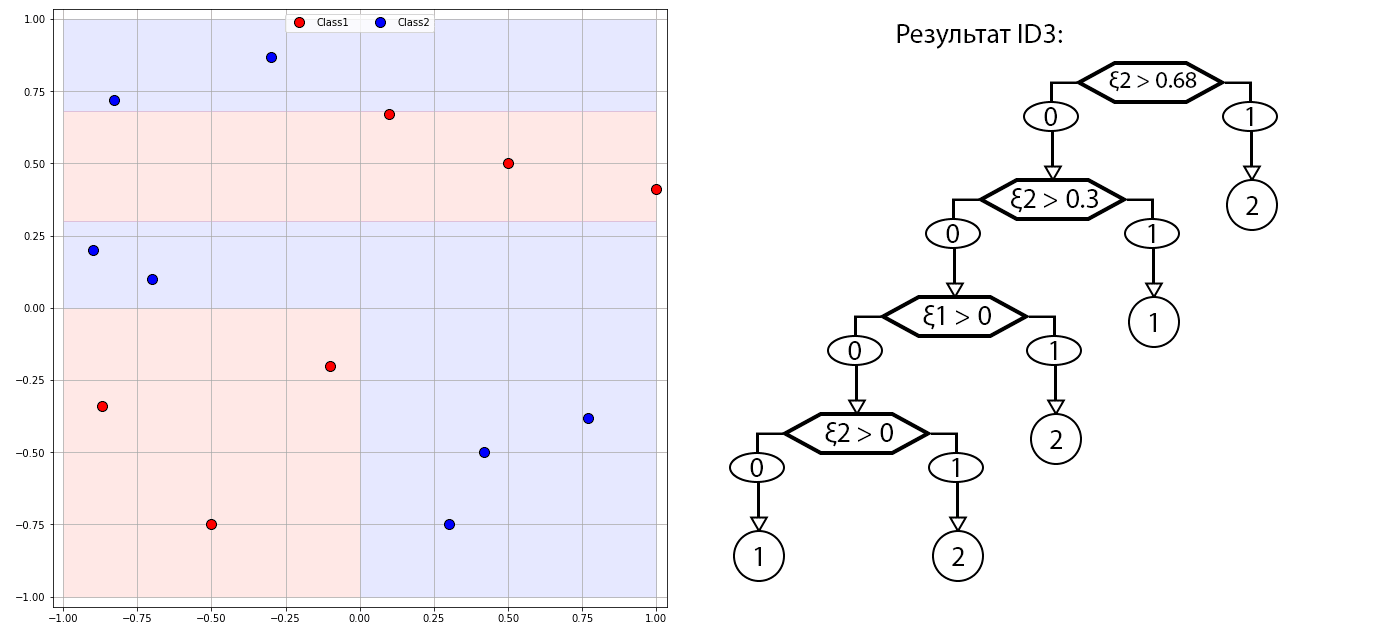
\includegraphics[scale=0.345]{images/3_6_XOR_ID3.png}
\end{center}

Жадный алгоритм стремится отделить два класса, а не разделить выборки поровну, где и там, и там будет примерно одинаковое количество объектов из каждого класса, чтобы только на следующем уровне разделить их окончательно. Таким образом, двухуровневое дерево жадным алгоритмом в данном случае никак не построить.
\\

Как бороться с такой ситуацией?

\subsubsection{Усечение дерева (pruning). Алгоритм C4.5}

Данный подход один из самый удачных и прижившихся. Он вошел в состав процедуры C4.5, которая имеет свободнодоступную реализацию (выложена в интернете). Алгоритм был предложен тем же автором, что и создал ID3.
\\

\textbf{Идея} следующая: если наша проблема заключается в переобучении и переусложнении структуры дерева, значит нам нужна \textit{контрльная выборка данных} для оценки \textit{обобщающей способности}.

Можно было бы делать это в процессе постройки дерева, но в данном случае алгоритм работает уже над построенным деревом.
\\

Мы разобьем обучающую выборку на две части: \textit{обучающую} и \textit{контрольную} --- обычно это делают в соотношении 2:1, но можно любое, например:

\begin{itemize}
\item[] $\qquad X^k$ --- независимая контрольная выборка, $k \approx 0.5l$.
\end{itemize}

Далее давайте опишем сам алгоритм, зная, что у нас уже есть построенное дерево и контрольная выборка:

\begin{center}
\newpage
\line(1,0){400}
\end{center}

\begin{itemize}
\item[1:] \textcolor{blue}{для всех} $v \in V_\text{внутр}$

				

\item[3:] \qquad \textcolor{blue}{если} $S_v = \emptyset$ \textcolor{blue}{то}

\item[4:] \qquad \qquad \textcolor{blue}{вернуть}
				новый лист $v, c_v := Мажоритарный класс(U)$;
			
\item[5:] \qquad число ошибок при классификации $S_v$ четырьмя способами:
		
			\qquad \qquad $r(v)$ --- поддеревом, растущим из вершины $v$;
			
			\qquad \qquad $r_L(v)$ --- поддеревом левой дочерней вершины $L_v$;
			
			\qquad \qquad $r_R(v)$ --- поддеревом правой дочерней вершины $R_v$;

			\qquad \qquad $r_c(v)$ --- к классу $c \in Y$.


\item[6:] \qquad в зависимости от того, какое из них минимально:
		
			\qquad \qquad сохранить поддерево $v$;
			
			\qquad \qquad заменить поддерево $v$ поддеревом $L_v$;
			
			\qquad \qquad заменить поддерево $v$ поддеревом $R_v$;

			\qquad \qquad заменить поддерево $v$ листом
							$c_v := arg\ \underset{c \in Y}{min}\ r_c(v)$.
\end{itemize}

\begin{center}
\line(1,0){400}
\end{center}

Разберем данный алгоритм по пунктам:

\begin{itemize}
\item Пропускаем нашу контрольную выборку через дерево, и для каждой внутренней вершины сохраняем подмножество объектов, которые дошли до данной вершины.

\qquad \qquad 1: \textcolor{blue}{для всех} $v \in V_\text{внутр}$

\qquad \qquad 2: \qquad $S_v :=$ подмножество объектов $X^k$, дошедших до $v$;

\item Для каждой внутренней вершины постараемся понять, нужна она, или ее можно заменить на лист, или упростить поддерево, которое растет из этой внутренней вершины...

Если оказалось, что множество контрольных объектов, дошедших до данной вершины \textit{пусто}, то упростим ее и заменим её листовой вершиной, и выберем в этой листовой вершине тот класс, к которому относится большинство объектов \textit{обучающей выборки} (контрольных же сюда дошло ноль, так что только по обучающей выборке нам и остается делать выводы).

\qquad \qquad 3: \qquad \textcolor{blue}{если} $S_v = \emptyset$ \textcolor{blue}{то}

\qquad \qquad 4: \qquad \qquad \textcolor{blue}{вернуть}
				новый лист $v, c_v := Мажоритарный класс(U)$;
			
\item Дальше мы должны принять решение, чем можно было бы заменить эту внутреннюю вершину. Способов это выбрать много, но алгоритм усечения предусматривает только 4 варианта:

	\begin{itemize}
	\item мы оставляем поддерево \textit{без изменений};
	\item заменяем поддерево её же \textit{левым} поддеревом;
	\item заменяем поддерево её же \textit{правым} поддеревом;
	\item заменяем \textit{терминальной} вершиной.
	\end{itemize}

	Выбор из этих четырех вариантов, на самом-то деле, достаточно простой. Надо просто для каждого варианта классифицировать объекты контрольной выборки (точнее объекты $S_v$, для данной вершины мы уже обрезали недошедшие), и просто выбрать тот вариант, где \textit{число ошибок минимально}.

\qquad \qquad 5: \qquad число ошибок при классификации $S_v$ четырьмя способами:
		
			\qquad \qquad \qquad \qquad $r(v)$ --- поддеревом, растущим из вершины $v$;
			
			\qquad \qquad \qquad \qquad $r_L(v)$ --- поддеревом левой дочерней вершины $L_v$;
			
			\qquad \qquad \qquad \qquad $r_R(v)$ --- поддеревом правой дочерней вершины $R_v$;

			\qquad \qquad \qquad \qquad $r_c(v)$ --- к классу $c \in Y$.


\qquad \qquad 6: \qquad в зависимости от того, какое из них минимально:
		
			\qquad \qquad \qquad \qquad сохранить поддерево $v$;
			
			\qquad \qquad \qquad \qquad заменить поддерево $v$ поддеревом $L_v$;
			
			\qquad \qquad \qquad \qquad заменить поддерево $v$ поддеревом $R_v$;

			\qquad \qquad \qquad \qquad заменить поддерево $v$ листом
							$c_v := arg\ \underset{c \in Y}{min}\ r_c(v)$.
\end{itemize}

Таким образом мы можем вершину за вершиной упростить дерево. \textit{Порядок} просмотра вершин зависит от реализации, в целом он не принципиален (в плане того, что алгоритм не сломается).

\subsubsection{CART: деревья регрессии и классификации}

\textbf{CART} --- \textbf{C}lassification and \textbf{R}egression \textbf{T}ree.

В этом дереве тоже есть очень похожий на $ID3$ жадный рекурсивный алгоритм построения дерева, тоже применяются стратегии усечения, но алгоритм обобщен на случаи регрессии.
\\

Для регрессии используется следующее обобщение: $Y = \mathbb{R}, c_v \in \mathbb{R}$.

А в качестве \textit{критерия информативности} мы используем другой критерий. Самое простое и естественное --- это использовать \textit{критерий среднеквадратичной ошибки} (тот же, что и в методе наименьших квадратов):
\\

Пусть $U_v$ --- по-прежнему является множеством объектов обучающей выборки, дошедших до вершины $v$.

\textbf{Значения в терминальных вершинах} --- МНК-решение (усредним значение ответов на всех объектах):

$$c_v := \text{\^y}(U_v) = \frac{1}{|U_v|}\sum\limits_{x_i \in U_v} y_i$$

\textbf{Критерий информативности} --- среднеквадратичная ошибка

$$I(\beta, U_v) = \sum\limits_{x_i \in U_v}(\text{\^y}_i(\beta) - y_i)^2,$$

где \^y$_i(\beta) = \beta(x_i)\text{\^y}(U_{v1}) + (1 - \beta(x_i))\text{\^y}(U_{v0})$ --- прогноз после ветвления $\beta$ и разбиения $U_v = U_{v0} \sqcup U_{v1}$.

\textbf{WARN: плохо понятая часть, need help! }
То есть выбор предиката осуществляется по тому, насколько хорошо он будет классифицировать то дерево, которое будет состоять из вершины и двух поддеревьев $v0$ и $v1$ (каждое из которых имеет свое среднее значение), в которые мы будем отправлять наши объекты $x_i$ (выбор ветви зависит от результата предиката $\beta(x_i)$).

Так произойдет разбиение и процесс построения дерева пойдет рекурсивно.
\\

В итоге дерево регрессии строит \textbf{кусочно-постоянную функцию}, потому что в каждом листе ответ, который будет выдавать этот алгоритм, является константой (среднее значение). Это означает, что дерево регрессии разделило все пространство объектов на какие-то куски, и в каждом куске выдается свое константное значение.

\subsubsection{CART: критерий Minimal Cost-Complexity Pruning}

Возвращаясь к вопросу оптимизации структуры дерева, для \textbf{CART} придуман очень эффективный критерий, который позволяет упростить структуру дерева.
\\

Здесь можно выписать критерий, который состоит из двух частей. Первое --- это среднеквадратичная ошибка. Второе --- \textbf{штрафное слагаемое}. Таким образом получаем:

\begin{itemize}
\item Среднеквадратичная ошибка со штрафом за сложность дерева:

$$C_\alpha =
\sum\limits_{x_i = 1}^l(\text{\^y} - y_i)^2 + \alpha|V_\text{лист}| \rightarrow min$$

По сути \textit{штрафное слагаемое} в данном случае --- это \textit{количество листьев} в дереве, домноженное на какой-то коэффициент, который называется \textit{константой регуляризации}.
\end{itemize}

Таким образом, мы можем выделить следующие моменты минимизации данной величины:

\begin{itemize}
\item При увеличении $\alpha$ дерево последовательно упрощается.

Причем последовательность вложенных деревьев единственна (это строго доказываемый факт).

\item Из этой последовательности выбирается дерево с минимальной ошибкой на тестовой выборке (Hold-Out).

\item Для случая классификации используется аналогичная стратегия усечения, с критерием Джини.
\end{itemize}

\section{Резюме}

\textbf{Преимущества решающих деревьев:}

\begin{itemize}
\item интерпретируемость,
\item допускаются разнотипные данные,
\item возможность обхода пропусков;
\end{itemize}

\textbf{Недостатки решающих деревьев}

\begin{itemize}
\item переобучение,
\item фрагментация
\item неустойчивость к шуму, составу выборки, критерию;
\end{itemize}

\textbf{Способы устранения этих недостатков:}

\begin{itemize}
\item редукция,
\item композиции (леса) деревьев (\textit{в следующих лекциях}).
\end{itemize}
\end{document}
